\subsection{Comparison}

At this moment, we have understood and tested both strategies, and it is moment to contrast each other and highlight their differences.

First of all we plot together the frequency histograms for the final wealth distribution for both models.

\begin{figure}[h]
    \centering
    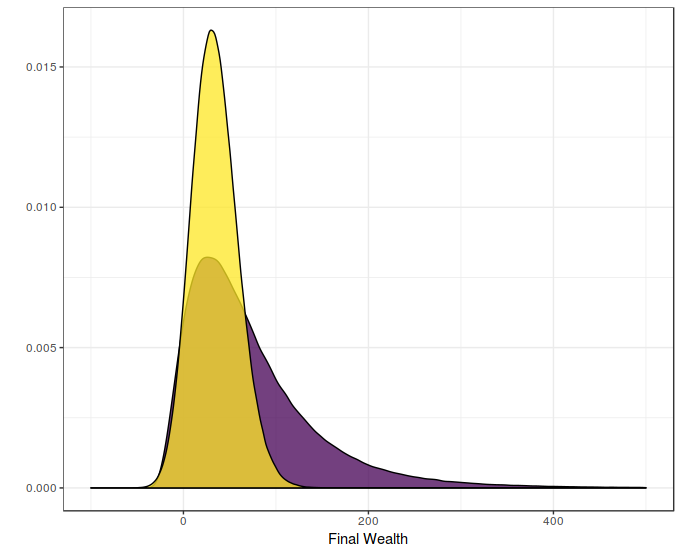
\includegraphics[scale=0.65]{./images/fw_both.png}
    \caption{Results of the simulation for the both models. Final wealth obtained for every simulation. The yellow one is the CPPI, and the purple one is the Alternative.}
    \label{fig:both_fw}
\end{figure}

Looking at Figure \ref{fig:both_fw} we may notice that they follow a considerably different distribution. We could say that the alternative strategy presents more dispersion, even though it is always a \textit{positive} deviation from the mean.

In section \ref{sec:risk} we have discussed a little bit some implications of the definition of risk. Affirm that the alternative strategy presents more risk, just because its result is more disperse, may seem a little simplistic.

On the other hand, we can take a look at those rare cases when the final wealth happens to be negative. These are the cases worth exploring, for it is the scenario every investor is afraid of: losing money. Zooming in into the negative zone, as shown in figure \ref{fig:loss_both}, we can focus in the difference between the two models. Even though we can see some spurious differences in some places, the most honest answer is that it is not clear whose result is less risky.

\begin{figure}[h]
    \centering
    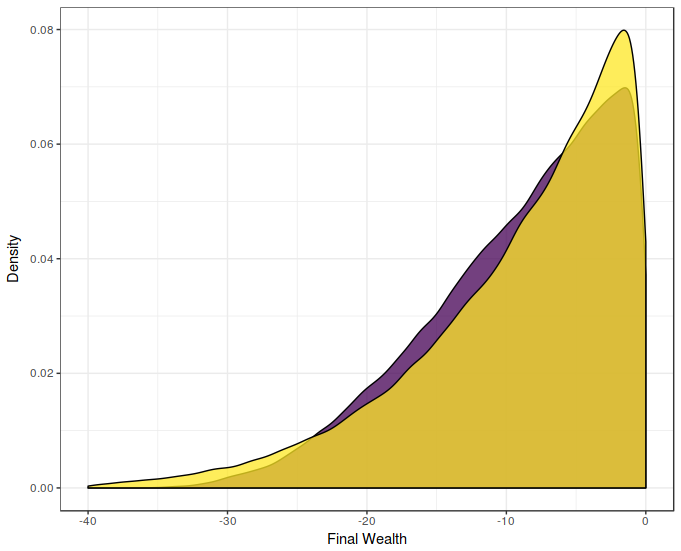
\includegraphics[scale=0.5]{./images/loss_both.png}
    \caption{Results of the simulation for the both models. Final wealth, filtered by negative values obtained for every simulation. The yellow one is the CPPI, and the purple one is the Alternative.}
    \label{fig:loss_both}
\end{figure}

In order to compare the degree of risk taken by every model, we make use of the \textit{Expected Shortfall}, as explained in section \ref{sec:risk}. If we set this parameter as the level of risk and we set it constant in both models, we can compare their returns. In~\cite{a:guillen-optimisation} it is shown that the Alternative model is able to set its Expected Shortfall (ES) by its $K$, using this formula:

\begin{align}\label{eq:kes}
	\frac{K}{ES} = \frac{1}{-1 + \qty(1 - \theta)^{-1} e^{\alpha A T}\Phi\qty(\Phi^{-1}\qty(1 - \theta) - A\sigma\sqrt{T})} \emph{.}
\end{align}

Where $\alpha$ is the expected return of the risky asset, $\sigma$ is the standard deviation of the risky asset, $\theta$ is the quantile on which the Expected Shortfall is measured, $A$ is the parameter that settles the risk aversion profile and $\Phi$ represents the standard Normal distribution function.

Therefore, the approach is the following: We set a constant proportion $\pi$ for the CPPI model, we simulate it many times and measure the ES for the results. Then we find the $K$ in order to set the same ES on the Alternative model. This way we can simulate both models making sure they will assume the same risk, and thus we can freely compare their returns.

Setting $\alpha = 0.343$, $\sigma = 0.1544$, $a = 10$, $T = 60$, $A = 0.5$ and number of simulations $N = 100,000$ we find the results shown in Table \ref{tab:cppi_alt}, in which we can see the outperformance of the alternative strategy, for many different levels of risk.

\begin{table}[h]
\centering
\caption{Results of $100,000$ simulations using different risk levels, with $\alpha = 0.343$, $\sigma = 0.1544$, $a = 10$, $T = 60$, $A = 0.5$ and therefore $ES/K = -3.3$. These results match approximately those presented in \cite{a:guillen-optimisation}, on Table 1 at page 8. Any differences are attributable to the intrinsic randomness of simulations.}
\label{tab:cppi_alt}
\begin{tabular}{ccccccc}
\textbf{$\pi$} & \textbf{ES } & \textbf{$K$} & \textbf{CPPI ret} & \textbf{Alt ret} & \textbf{diff}  & \textbf{equiv $\pi$}\\
0.1   & -12.47  & 40.59  & 0.33     & 0.51    & 0.18    & 0.17\\
0.2   & -27.03  & 87.98  & 0.65     & 0.98    & 0.38    & 0.30 \\
0.3   & -42.99  & 139.95 & 0.95     & 1.42    & 0.46    & 0.45 \\
0.4   & -60.13  & 195.71 & 1.23     & 1.83    & 0.60    & 0.61 \\
0.5   & -78.25  & 255.02 & 1.5      & 2.22    & 0.71    & 0.69 \\
0.6   & -99.96  & 325.36 & 1.76     & 2.63    & 0.87    & 0.92 \\
0.7   & -120.61 & 392.56 & 2.00     & 3.00    & 1.00    & * \\
0.8   & -144.71 & 471.02 & 2.23     & 3.40    & 1.17    & * \\
0.9   & -172.94 & 562.92 & 2.39     & 3.81    & 1.42    & * \\
1     & -205.09 & 667.57 & 2.58     & 4.27    & 1.70    & *
\end{tabular}
\end{table}

The interesting conclusion that can be extracted from Table \ref{tab:cppi_alt} is the value of the last column. It states the necessary value of $\pi$ that the CPPI should get in order to equal the return of the Alternative strategy, what we call the equivalent $\pi$. Thus, if the Expected Shortfall was settled by some $\pi$ and the required equivalent $\pi$ is greater than that, we are saying that the CPPI should undertake in more risk in order to equal the return of the Alternative Scheme.

This equivalent $\pi$ thus works as a succint metric to compare the performance of this two strategies, taking into account both return and risk. Hence, as long as the equivalent $\pi$ is greater than the initial $\pi$, we can say that the Alternative Strategy is outperforming the CPPI. Which is clear for many values of initial $\pi$ and a fixed value for $A$.

However, in Figure \ref{fig:pi-A_all-pis} we can show the iterated simulation of Table \ref{tab:cppi_alt}, for many different values of $\pi$ and many values of $A$. It is quite interesting to notice how this \emph{outperformance} occurs whilst the continuous line is above the dashed line. And their downhill tendency suggests that the Alternative Strategy is more worth ir for smaller values of $A$.

Since the value of $A$ is interpreted as the inverse of the risk aversion~\cite{a:guillen-optimisation} of the investor, we could argue that the riskier the inversor the less worth it the Alternative Scheme becomes, until a point (usually around $A = 1.5$) where the CPPI is outperforming the Alternative Strategy. Interestingly enough, this point is the same for all values of initial $\pi$. Indicating that, regardless of the chosen value for $\pi$ the decision upon the election of one of the strategies relies on the risk aversion profile of each investor.


\begin{figure}[h]
    \centering
    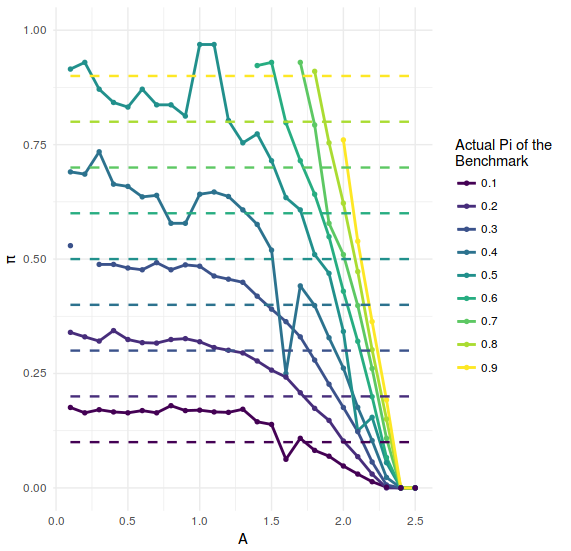
\includegraphics[scale=0.75]{./images/pi-A-all-pis.png}
    \caption{Plot that shows the relation between equivalent $\pi$ and $A$, for many different initial $\pi$. From the results of $100,000$ simulations for each curve, with $\alpha = 0.343$, $\sigma = 0.1544$, $a = 10$, $T = 60$.}
    \label{fig:pi-A_all-pis}
\end{figure}


It is important to highlight that all the deductions derived from the study of these results is a consequence of the assumption that the Expected Shortfall of both schemes is equalise for each value of $\pi$. As concluded by Equation~\ref{eq:kes}. Just to double-check, we have measured that this holds true for all simulations partaken in the results shown in Figure \ref{fig:es-es_pi2}. We might notice a slight deviation from that when the Expected Shortfall approaches 0, but nothing that could undermine the conclusions deduced from these results.


\begin{figure}[h]
    \centering
    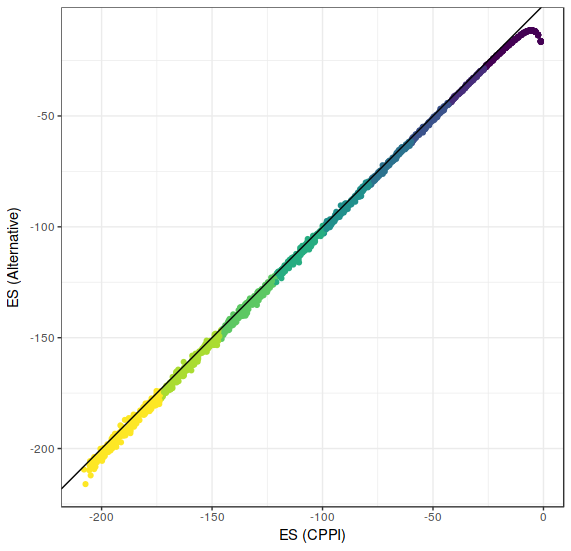
\includegraphics[scale=0.75]{./images/es-es_pi.png}
    \caption{Scatterplot that shows the equivalence between the Expected Shortfall derived from the simulations of Figure \ref{fig:pi-A_all-pis}. With $\alpha = 0.343$, $\sigma = 0.1544$, $a = 10$, $T = 60$.}
    \label{fig:es-es_pi}
\end{figure}


\begin{figure}
\centering
\begin{subfigure}{.5\textwidth}
    \centering
    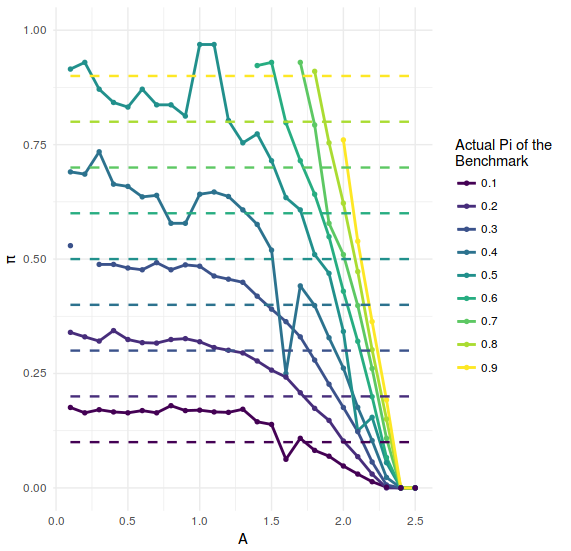
\includegraphics[scale=0.5]{./images/pi-A-all-pis.png}
    \caption{Plot that shows the relation between equivalent $\pi$ and $A$.}
    \label{fig:pi-A_all-pis2}
\end{subfigure}%
\begin{subfigure}{.5\textwidth}
    \centering
    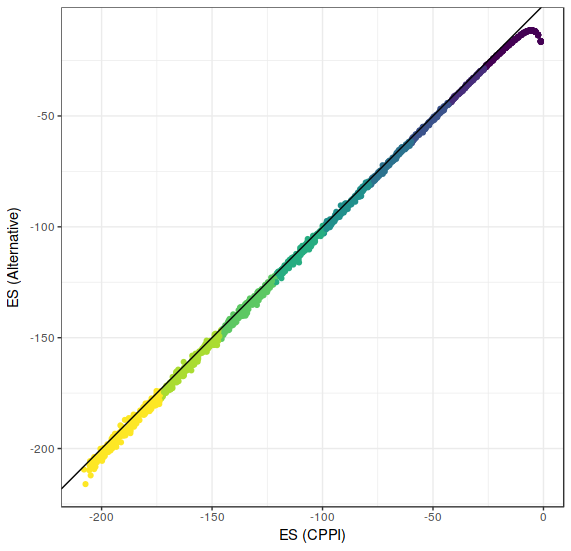
\includegraphics[scale=0.5]{./images/es-es_pi.png}
    \caption{Scatterplot that shows the equivalence between the Expected Shortfall derived from the simulations of Figure \ref{fig:pi-A_all-pis2}.}
    \label{fig:es-es_pi2}
\end{subfigure}
\caption{Results from $20,000,000$ simulations performed for many different values of $\pi$ and $A$, with $\alpha = 0.343$, $\sigma = 0.1544$, $a = 10$, $T = 60$.}
\label{fig:test}
\end{figure}


